\documentclass{report}
\usepackage{hyperref}
\usepackage{geometry}
\usepackage{scalerel,amssymb}
\usepackage{paralist}
\usepackage{amsmath}
\usepackage{pgfplots}
\usepackage{tikz}
\usetikzlibrary{positioning}
\usetikzlibrary{shapes.geometric, arrows}
\tikzstyle{arrow} = [thick,->,>=stealth]

\usepackage{stackengine}
\def\apeqA{\SavedStyle\sim}
\def\apeq{\setstackgap{L}{\dimexpr.5pt+1.5\LMpt}\ensurestackMath{%
  \ThisStyle{\mathrel{\Centerstack{{\apeqA} {\apeqA} {\apeqA}}}}}}

\begin{document}
\begin{center}
\huge{\textbf{\underline{Cryptography}}}
\end{center}


{\let\clearpage\relax \chapter*{5. Pseudorandom Generators}}
	\section*{5.1 Introduction}
		A pseudorandom generator(PRG) is a deterministic function that
		\begin{enumerate}[-]
			\item stretches a "short", truly random input (seed) to a long sequence  of \underline{pseudorandom} bits
			\item directly gives a \underline{stream cipher}
			\item perhaps the most basic toll of cryptography
		\end{enumerate}
		\subsection*{Definition:}
			A PRG is a deterministic function $G: \{ 0,1 \} ^{\lambda} \rightarrow \{ 0,1 \} ^{\lambda + l}$ that satisfies: \\ \\
			\begin{tabular}{lll}
				\begin{tabular}{l}
					$L_{PRG-real}$ \\
					\hline \underline{$Query():$} \\
					\ $s \textit{ (seed) } \leftarrow \{ 0,1 \} ^{\lambda}$ \\
					\ \underline{return} G(s) \\ \hline
				\end{tabular}	
				&
				&
				\begin{tabular}{l}
					$L_{PRG-rand}$ \\
					\hline \underline{$Query():$} \\
					\ $r \leftarrow \{ 0,1 \} ^{\lambda + l}$ \\
					\ \underline{return} r \\ \hline
				\end{tabular}					
			\end{tabular}
		\subsection*{Example:}
			A length-doubling PRG:
			\begin{align*}		
				G:\{ 0,1 \} ^{\lambda} \ & \rightarrow \ \{ 0,1 \} ^{2 \lambda} \\
				\mid dom(G) \mid \ & = \ 2^{\lambda} \\
				\mid range(G) \mid \ & \leq \ 2^{2\lambda}
			\end{align*}
		
			\begin{enumerate}[\textbullet]
				\item Even if $G(s)$ for random $s \leftarrow \{ 0,1 \} ^{\lambda}$ outputs only a small subset of $\{ 0,1 \} ^{2\lambda}$, no efficient (ppt) algorithm can distinguish $G(s)$ from a truly random $2\lambda$-bit string.
			\end{enumerate}
\newpage
		\subsection*{(Counter-)Example:}
			Java: java.util.random \\
			$\star$ new Random(seed s) \\
			linear congruential generator:
			\begin{align*}
				s_0 \ & := \ seed \\
				s_{i+1} \ & := \ (s_i \cdot a +c) mod n
			\end{align*}
			\textsc{Insecure:} NOT A PRG !!!
		
	\section*{5.3 Stream cipher - Encryption from a PRG}
		\begin{enumerate}[\textbullet]
			\item A stream cipher performs encryption like the OTP, but:
			\begin{enumerate}[-]
				\item uses a short key
				\item with computational security (conditional security)
			\end{enumerate}
			\item Prototype for a symmetric cryptosystem; also fastest
		\end{enumerate}
		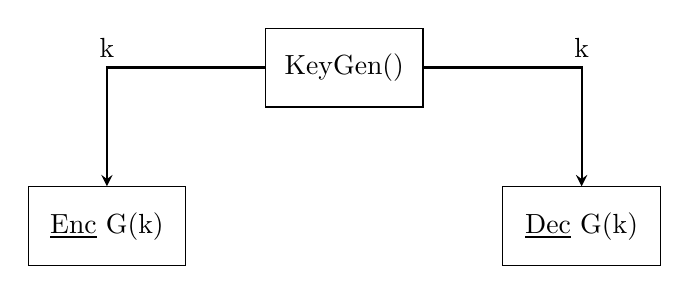
\begin{tikzpicture}
			%Nodes
			\node (rect) [draw,thin,minimum width=2cm,minimum height=1cm] (KeyGen) {KeyGen()};
			\node (rect) [draw,thin,minimum width=2cm,minimum height=1cm, below left=of KeyGen] (Enc) {\underline{Enc} G(k)};
			\node (rect) [draw,thin,minimum width=2cm,minimum height=1cm, below right=of KeyGen] (Dec) {\underline{Dec} G(k)};
			
			%Lines
			\draw[arrow] (KeyGen.west) -| node[ anchor=south ]{k} (Enc.north);
			\draw[arrow] (KeyGen.east) -| node[ anchor=south ]{k} (Dec.north);
		\end{tikzpicture}
		\subsection*{Remarks}
		\begin{enumerate}[\textbullet]
			\item Encryption and decryption are stateful
			\item Requires PRG outputs the key stream in pieces
			\item Stream cipher directly malleable and provides no integrity or authenticity \\
				$\rightarrow$ needs additional tools to ensure integrity ($\rightarrow$ MAC)
		\end{enumerate}
\newpage
	\section*{One-time encryption with computational security}
		\subsection*{Definition}
		An encritpion scheme $\Sigma \ = \ (KeyGen, \ Enc, \ Dec)$ has computational one-time secrecy if
		\[
			L_{ots-L}^{\Sigma} \ \stackrel{\sim}{\approx} \ L_{ots-R}^{\Sigma}
		\]
		\begin{tabular}{lll}
			\begin{tabular}{l}
				$L_{ots-L}$ \\
				\hline \underline{$Eavesdrop(m_L,m_R):$} \\
				\ $k \leftarrow \Sigma . KeyGen()$ \\
				\ $c := \Sigma .Enc(k,m_L)$ \\
				\ \underline{return} c \\ \hline
			\end{tabular}	
			&
			&
			\begin{tabular}{l}
				$L_{ots-R}$ \\
				\hline \underline{$Eavesdrop(m_L,m_R):$} \\
				\ $k \leftarrow \Sigma . KeyGen()$ \\
				\ $c := \Sigma .Enc(k,m_R)$ \\
				\ \underline{return} c \\ \hline
			\end{tabular}					
		\end{tabular}
		\subsection*{Stream cipher s using a PRG G}
			\begin{align*}
				K \ & = \ \{ 0,1 \} ^{\lambda} \\
				M \ & = \ \{ 0,1 \} ^{\lambda + l} \\
				C \ & = \ \{ 0,1 \} ^{\lambda + l} \\
			\end{align*}
			\begin{tabular}{lllll}
				\begin{tabular}{l}
					\underline{$KeyGen():$} \\
					\ $k \leftarrow \{ 0,1 \} ^{\lambda}$ \\
					\ \underline{return} k
				\end{tabular}	
				&
				&
				\begin{tabular}{l}
					\underline{$Enc(k, m):$} \\
					\ \underline{return} $G(k) \oplus m$
				\end{tabular}
				&
				&
				\begin{tabular}{l}
					\underline{$Enc(k, m):$} \\
					\ \underline{return} $G(k) \oplus c$
				\end{tabular}					
			\end{tabular}
		\subsection*{Theorem:}
			\underline{If} G is a secure PRG, \underline{then} stream cipher s has computational one-time secrecy:
			\[
				i.e. \ L_{ots-L}^{\Sigma} \ \apeq \ L_{ots-R}^{\Sigma}
			\]
			
		\begin{tabular}{lllll}
			\begin{tabular}{l}
				$L_{ots-L}$ \\
				\hline \underline{$Eavesdrop(m_L,m_R):$} \\
				\ $k \leftarrow \Sigma . KeyGen()$ \\
				\ $c := \Sigma .Enc(k,m_L)$ \\
				\ \underline{return} c \\ \hline
			\end{tabular}	
			&
			$\equiv$
			&
			\begin{tabular}{l}
				\underline{$Eavesdrop(m_L,m_R):$} \\
				\ $k \leftarrow \{ 0,1 \} ^{\lambda}$ \\
				\ $c := G(k) \oplus m_L$ \\
				\ \underline{return} c \\ \hline
			\end{tabular}
			&
			$\equiv$
			&
			\begin{tabular}{l}
				\underline{$Eavesdrop(m_L,m_R):$} \\
				\ $k \leftarrow \{ 0,1 \} ^{\lambda}$ \\
				\ z := G(k) \\
				\ $c := z \oplus m_L$ \\
				\ \underline{return} c \\ \hline
			\end{tabular}				
		\end{tabular}
		\hfill \\
		\begin{tabular}{llllll}
			$\apeq$
			&
			\begin{tabular}{l}
				\underline{$Eavesdrop(m_L,m_R):$} \\
				\ $z \leftarrow \{ 0,1 \} ^{\lambda + l}$ \\
				\ $c := z \oplus m_L$ \\
				\ \underline{return} c \\ \hline
			\end{tabular}	
			&
			$\equiv$
			&
			\begin{tabular}{l}
				\underline{$Eavesdrop(m_L,m_R):$} \\
				\ $z \leftarrow \{ 0,1 \} ^{\lambda + l}$ \\
				\ $c := z \oplus m_R$ \\
				\ \underline{return} c \\ \hline
			\end{tabular}
			&
			$\apeq$
			&
			\begin{tabular}{l}
				\underline{$Eavesdrop(m_L,m_R):$} \\
				\ $k \leftarrow \{ 0,1 \} ^{\lambda}$ \\
				\ z := G(k) \\
				\ $c := z \oplus m_R$ \\
				\ \underline{return} c \\ \hline
			\end{tabular}		
		\end{tabular}
		\hfill \\
		\begin{tabular}{llll}
			$\equiv$
			&
			\begin{tabular}{l}
				\underline{$Eavesdrop(m_L,m_R):$} \\
				\ $k \leftarrow \{ 0,1 \} ^{\lambda}$ \\
				\ $c := G(k) \oplus m_R$ \\
				\ \underline{return} c \\ \hline
			\end{tabular}
			&
			$\equiv$
			&
			\begin{tabular}{l}
				$L_{ots-R}$ \\
				\hline \underline{$Eavesdrop(m_L,m_R):$} \\
				\ $k \leftarrow \Sigma . KeyGen()$ \\
				\ $c := \Sigma .Enc(k,m_R)$ \\
				\ \underline{return} c \\ \hline
			\end{tabular}				
		\end{tabular}
		
	\section*{5.5 Extending the stretch of a PRG}
		\begin{enumerate}
			\item A length-doubling PRG \\ \\
			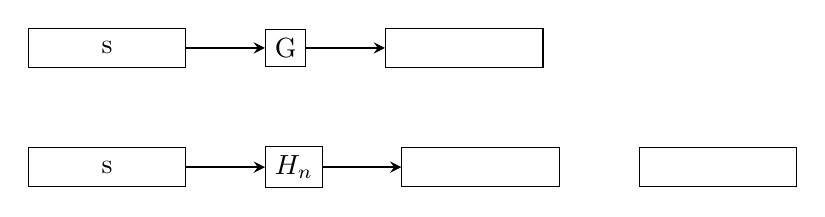
\begin{tikzpicture}
				%Nodes
				\node (rect) [draw,thin,minimum width=2cm,minimum height=0.5cm] (s1) {s};
				\node (rect) [draw,thin,minimum width=0.1cm,minimum height=0.1cm, right=of s1] (G) {G};
				\node (rect) [draw,thin,minimum width=2cm,minimum height=0.5cm, right=of G] (rect1) {};
				
				\node (rect) [draw,thin,minimum width=2cm,minimum height=0.5cm, below=of s1] (s2) {s};
				\node (rect) [draw,thin,minimum width=0.1cm,minimum height=0.1cm, right=of s2] (H) {$H_n$};
				\node (rect) [draw,thin,minimum width=2cm,minimum height=0.5cm, right=of H] (rect2) {};
				\node (rect) [draw,thin,minimum width=2cm,minimum height=0.5cm, right=of rect2] (rect3) {};
			
				%Lines
				\draw[arrow] (s1.east) -- (G.west);
				\draw[arrow] (G.east) -- (rect1.west);
				
				\draw[arrow] (s2.east) -- (H.west);
				\draw[arrow] (H.east) -- (rect2.west);
			\end{tikzpicture}
			\item Extension of length doubling G to (n+1) fold expansion:
			\begin{tabular}{l}
				\begin{tabular}{l}
					\underline{$H_n(s \in \{ 0,1 \} ^{\lambda})$} \\
					\ $s_0 := s$ \\
					\ \underline{for} $i := 1,...,n$ \underline{do} \\
					\ \ $t_i \| s_i := G(s_{i-1}$ \\
					\ \underline{return} $t_i \| ... \| t_n \| s_n$
				\end{tabular}
			\end{tabular}			
		\end{enumerate}
		We want to show: \\ \\
		\begin{tabular}{lll}
			\begin{tabular}{l}
				$L_{PRG-real}^{H}$ \\
				\hline \underline{$Query():$} \\
				\ $s \textit{ (seed) } \leftarrow \{ 0,1 \} ^{\lambda}$ \\
				\ \underline{return} $H_n(s)$ \\ \hline
			\end{tabular}	
			&
			$\apeq$
			&
			\begin{tabular}{l}
				$L_{PRG-rand}^{H}$ \\
				\hline \underline{$Query():$} \\
				\ $r \leftarrow \{ 0,1 \} ^{\lambda + l}$ \\
				\ \underline{return} r \\ \hline
			\end{tabular}					
		\end{tabular}

\end{document}
 